%! TEX root = ../main.tex
\documentclass[../main.tex]{subfiles}

\begin{document}

\subsection{Fenditura da $\mathbf{\qty{0.02}{\mm}}$}

Per la fenditura da $\qty{0.02}{\mm}$ ed apertura del sensore pari a $\qty{1.5}{\mm}$ sono stati raccolti $4$ set di dati che sono riportati in %\autoref{}.

\begin{figure}[ht!]
    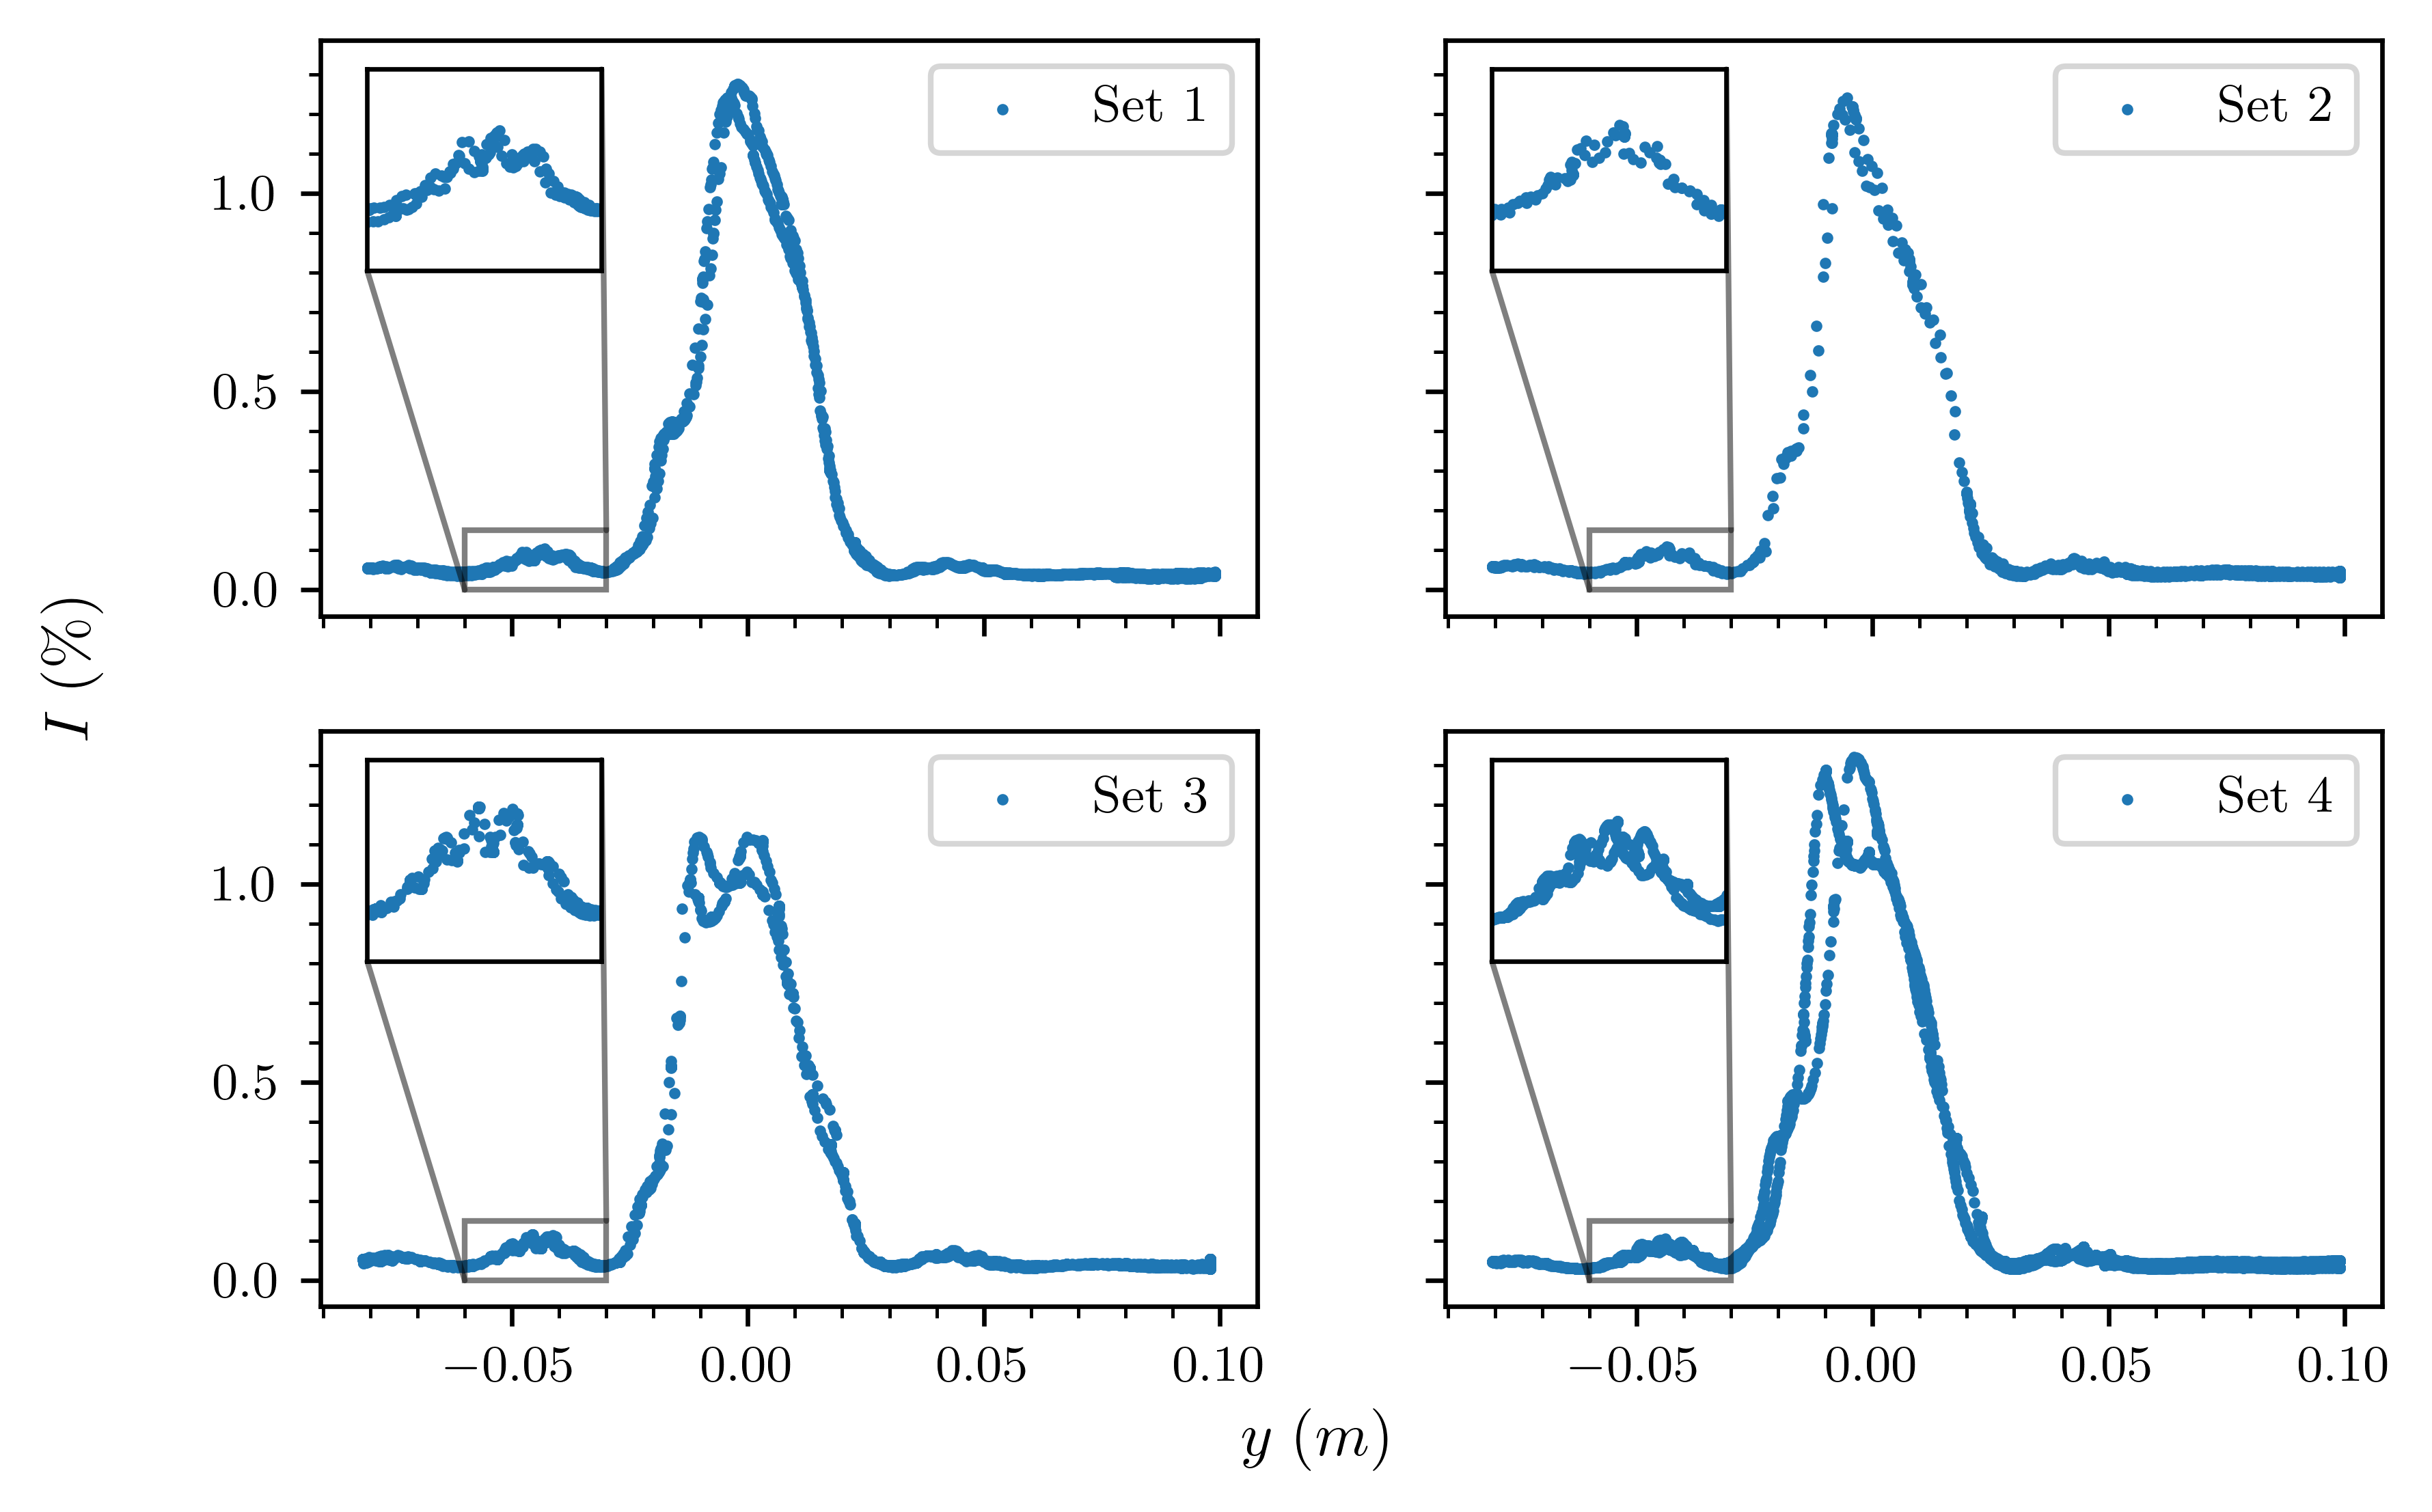
\includegraphics{single_scatter_0.02.png}
    \caption{Misure dell'intensità luminosa $I$ in funzione della posizione $y$ (in metri) del sensore. In tutti i set è possibile notare una deformazione del picco centrale che tende verso sinistra, a partire dal Set $3$ è possibile ipotizzare la presenza di un segnale a frequenza costante che si sovrappone alla figura di diffrazione causando una biforcazione del picco centrale. La presenza di un segnale "parassita" è visibile anche nelle code della curva, il fenomeno è maggiormente visibile in \autoref{fig:minimi 0.02}. Infine è presente una asimmetria nelle code per cui l'intensità luminosa risulta essere maggiore a sinistra.}
    \label{fig:single scatter 0.02}
\end{figure}

\begin{figure}[ht!]
    \centering
    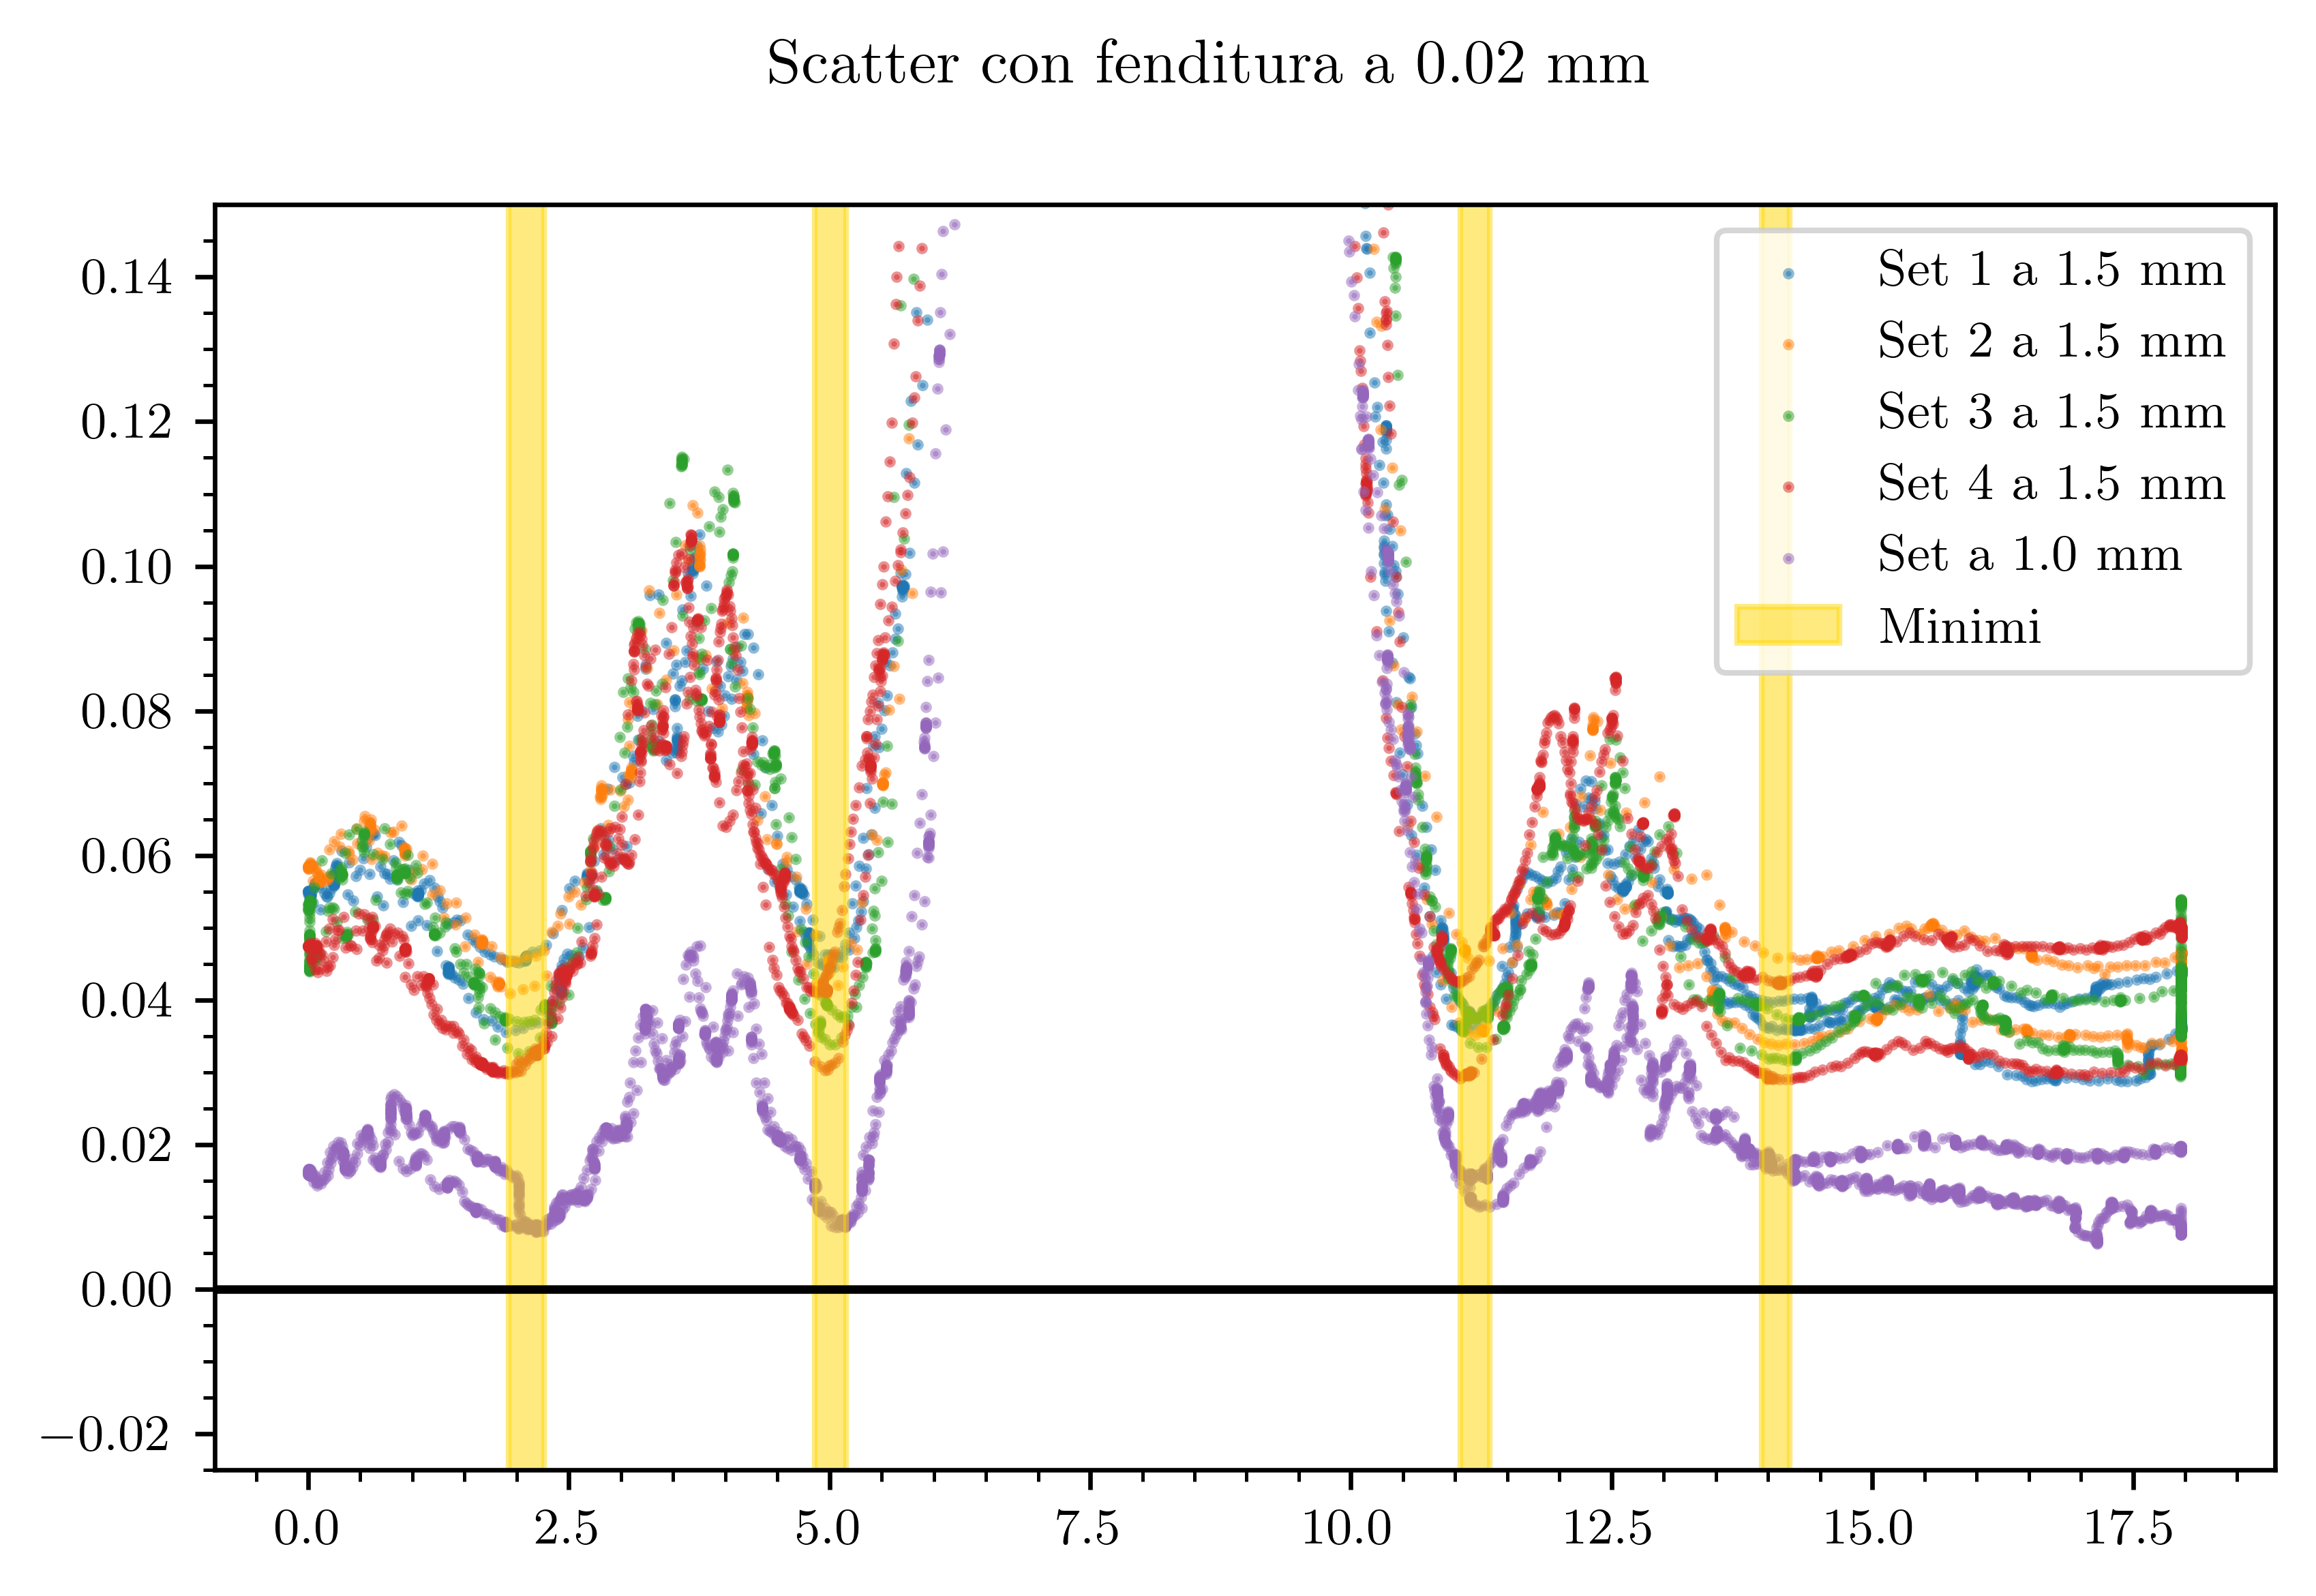
\includegraphics{min_0.02.png}
    \caption{Intensità luminosa $I$ in funzione della posizione $y$ del sensore (in metri) per la fenditura a $\qty{0.02}{\milli\metre}$. Si può notare un'asimmetria dei picchi  rispetto al centro. In figura sono segnati i minimi ricavati graficamente con i relativi errori. Su ciascun minimo si considera un errore di posizione di $\qty{1.0}{\mm}$, che contribuisce all'ampiezza di ciascuno degli intervalli evidenziati. È possibile notare un segnale a frequenza costante che si sovrappone alla figura di diffrazione.} % todo: aggiungere qualcosa in più alla descrizione+ commento asimmetria dati?
    \label{fig:minimi 0.02}
\end{figure}

Le posizioni dei minimi ottenute dalla \autoref{fig:minimi 0.02} sono riportate in \autoref{tab:minimi 0.02}.

\begin{table}[ht!]
    \centering
    \caption{Posizione dei minimi, ottenuta graficamente dalla \autoref{fig:minimi 0.02}, riportata di fianco al proprio indice $m$ ed al valore $\frac{\lambda L}{a} \; (\si{\metre})$ stimati seguendo l'\autoref{eq:y=0 values}. Il valore di $a$ derivato da ciascun minimo è stato ricavato con la formula inversa dopo aver posto $\lambda = \qty{650}{\nm}$ ed $L = \qty{98.5+-0.1}{\cm}$ sommando in quadratura i contributi all'errore di $\delta y$ e $\delta L$.}
    \import{../tables/}{mins_0.02.tex}
    \label{tab:minimi 0.02}
\end{table}

Intersecando i valori di $a$ così ricavati si ottiene $a = \qty{0.021+-0.002}{\mm}$.

% Facendo una media pesata dei valori di $a$ ottenuti si ottiene $a = \qty{0.0209+-0.0012}{\mm}$. %? review: è meglio l'intersezione o la media?

\begin{figure}[ht!]
    \centering
    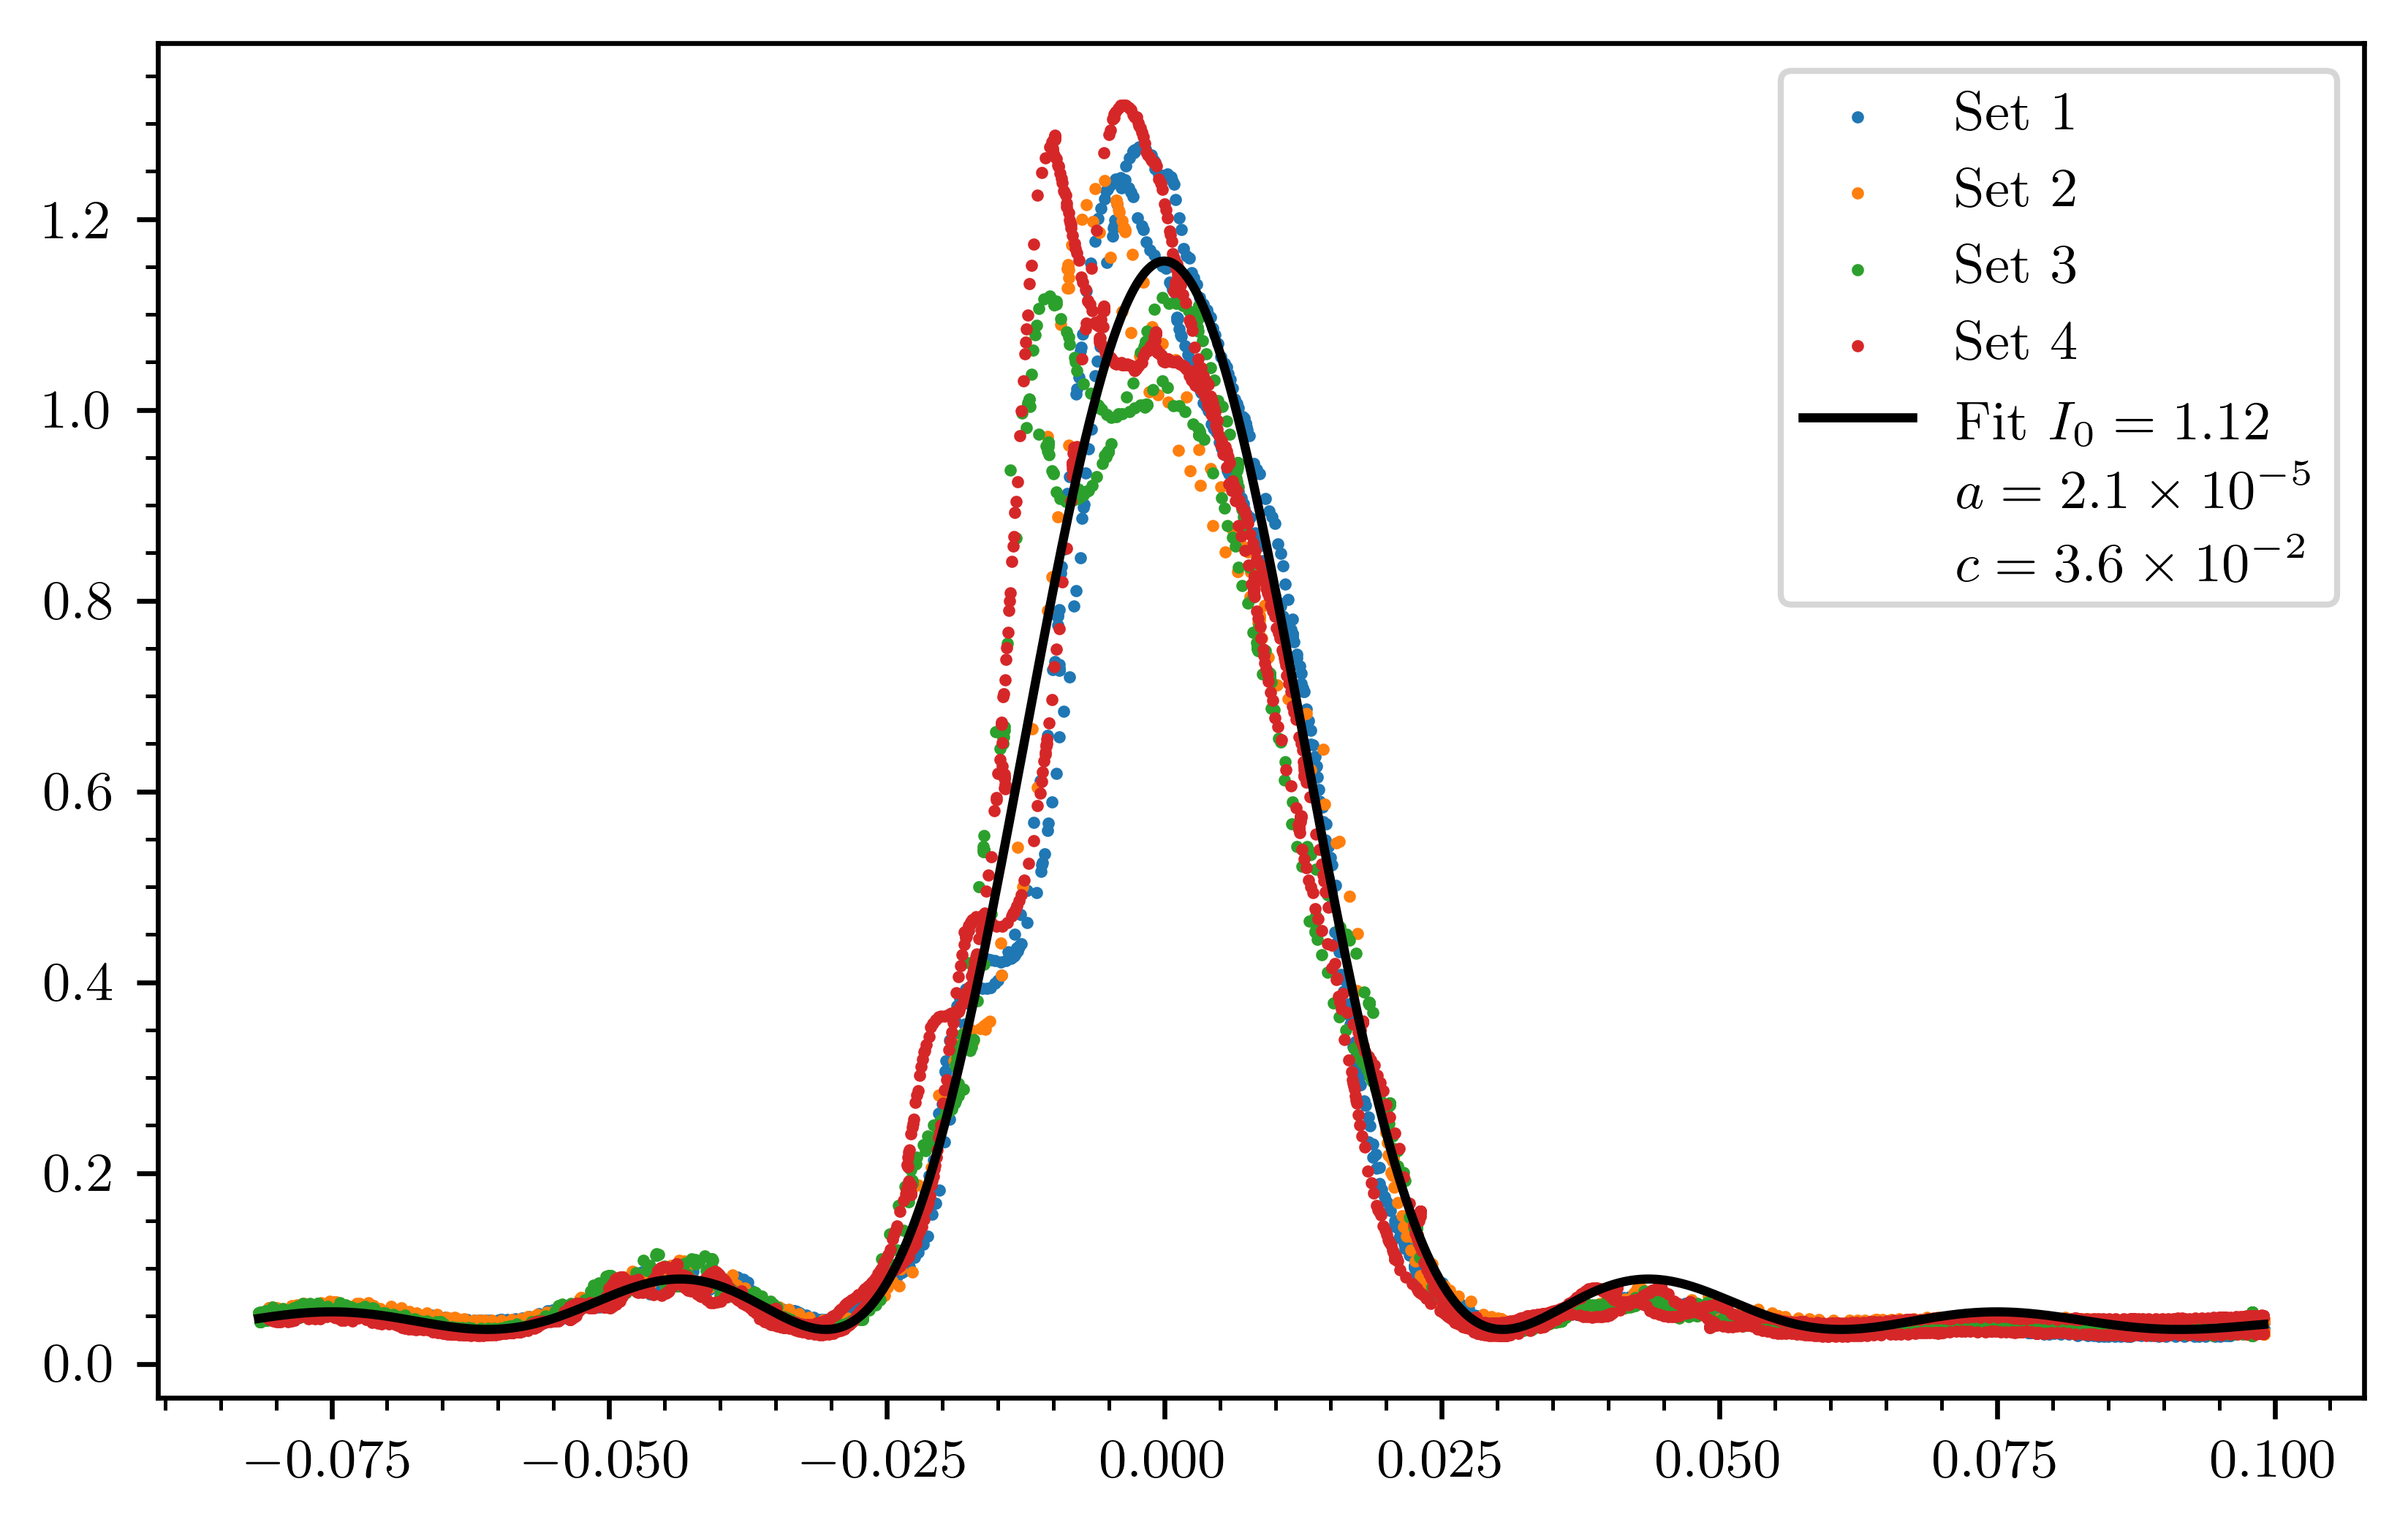
\includegraphics{fit_0.02.png}
    \caption{Intensità luminosa $I_{0}$ in funzione della posizione $y$ del sensore (in metri) per la fenditura a $\qty{0.02}{\mm}$. In figura è riportato il fit fatto utilizzando l'\autoref{eq:fit}. I valori dei parametri ottenuti sono $I_{0} = \num{1.12+-0.15}$, $a = \qty{0.021+-0.002}{\mm}$ e $c = \num{3.6+-0.8e-2}$.}
    \label{fig:fit 0.02}
\end{figure}

Sia il valore ottenuto col fit che il valore ottenuto dal grafico risultano compatibili con il valore teorico di $a$.

Per confrontare le misure ottenute con diverse aperture del sensore si è scelto di utilizzare il set $1$ delle misure con apertura $\qty{1.5}{\mm}$, in quanto è quello che meno presenta deformazioni lungo il picco centrale e ci permette di confrontare l'ampiezza di quest'ultimo.

\begin{figure}[ht!]
    \centering
    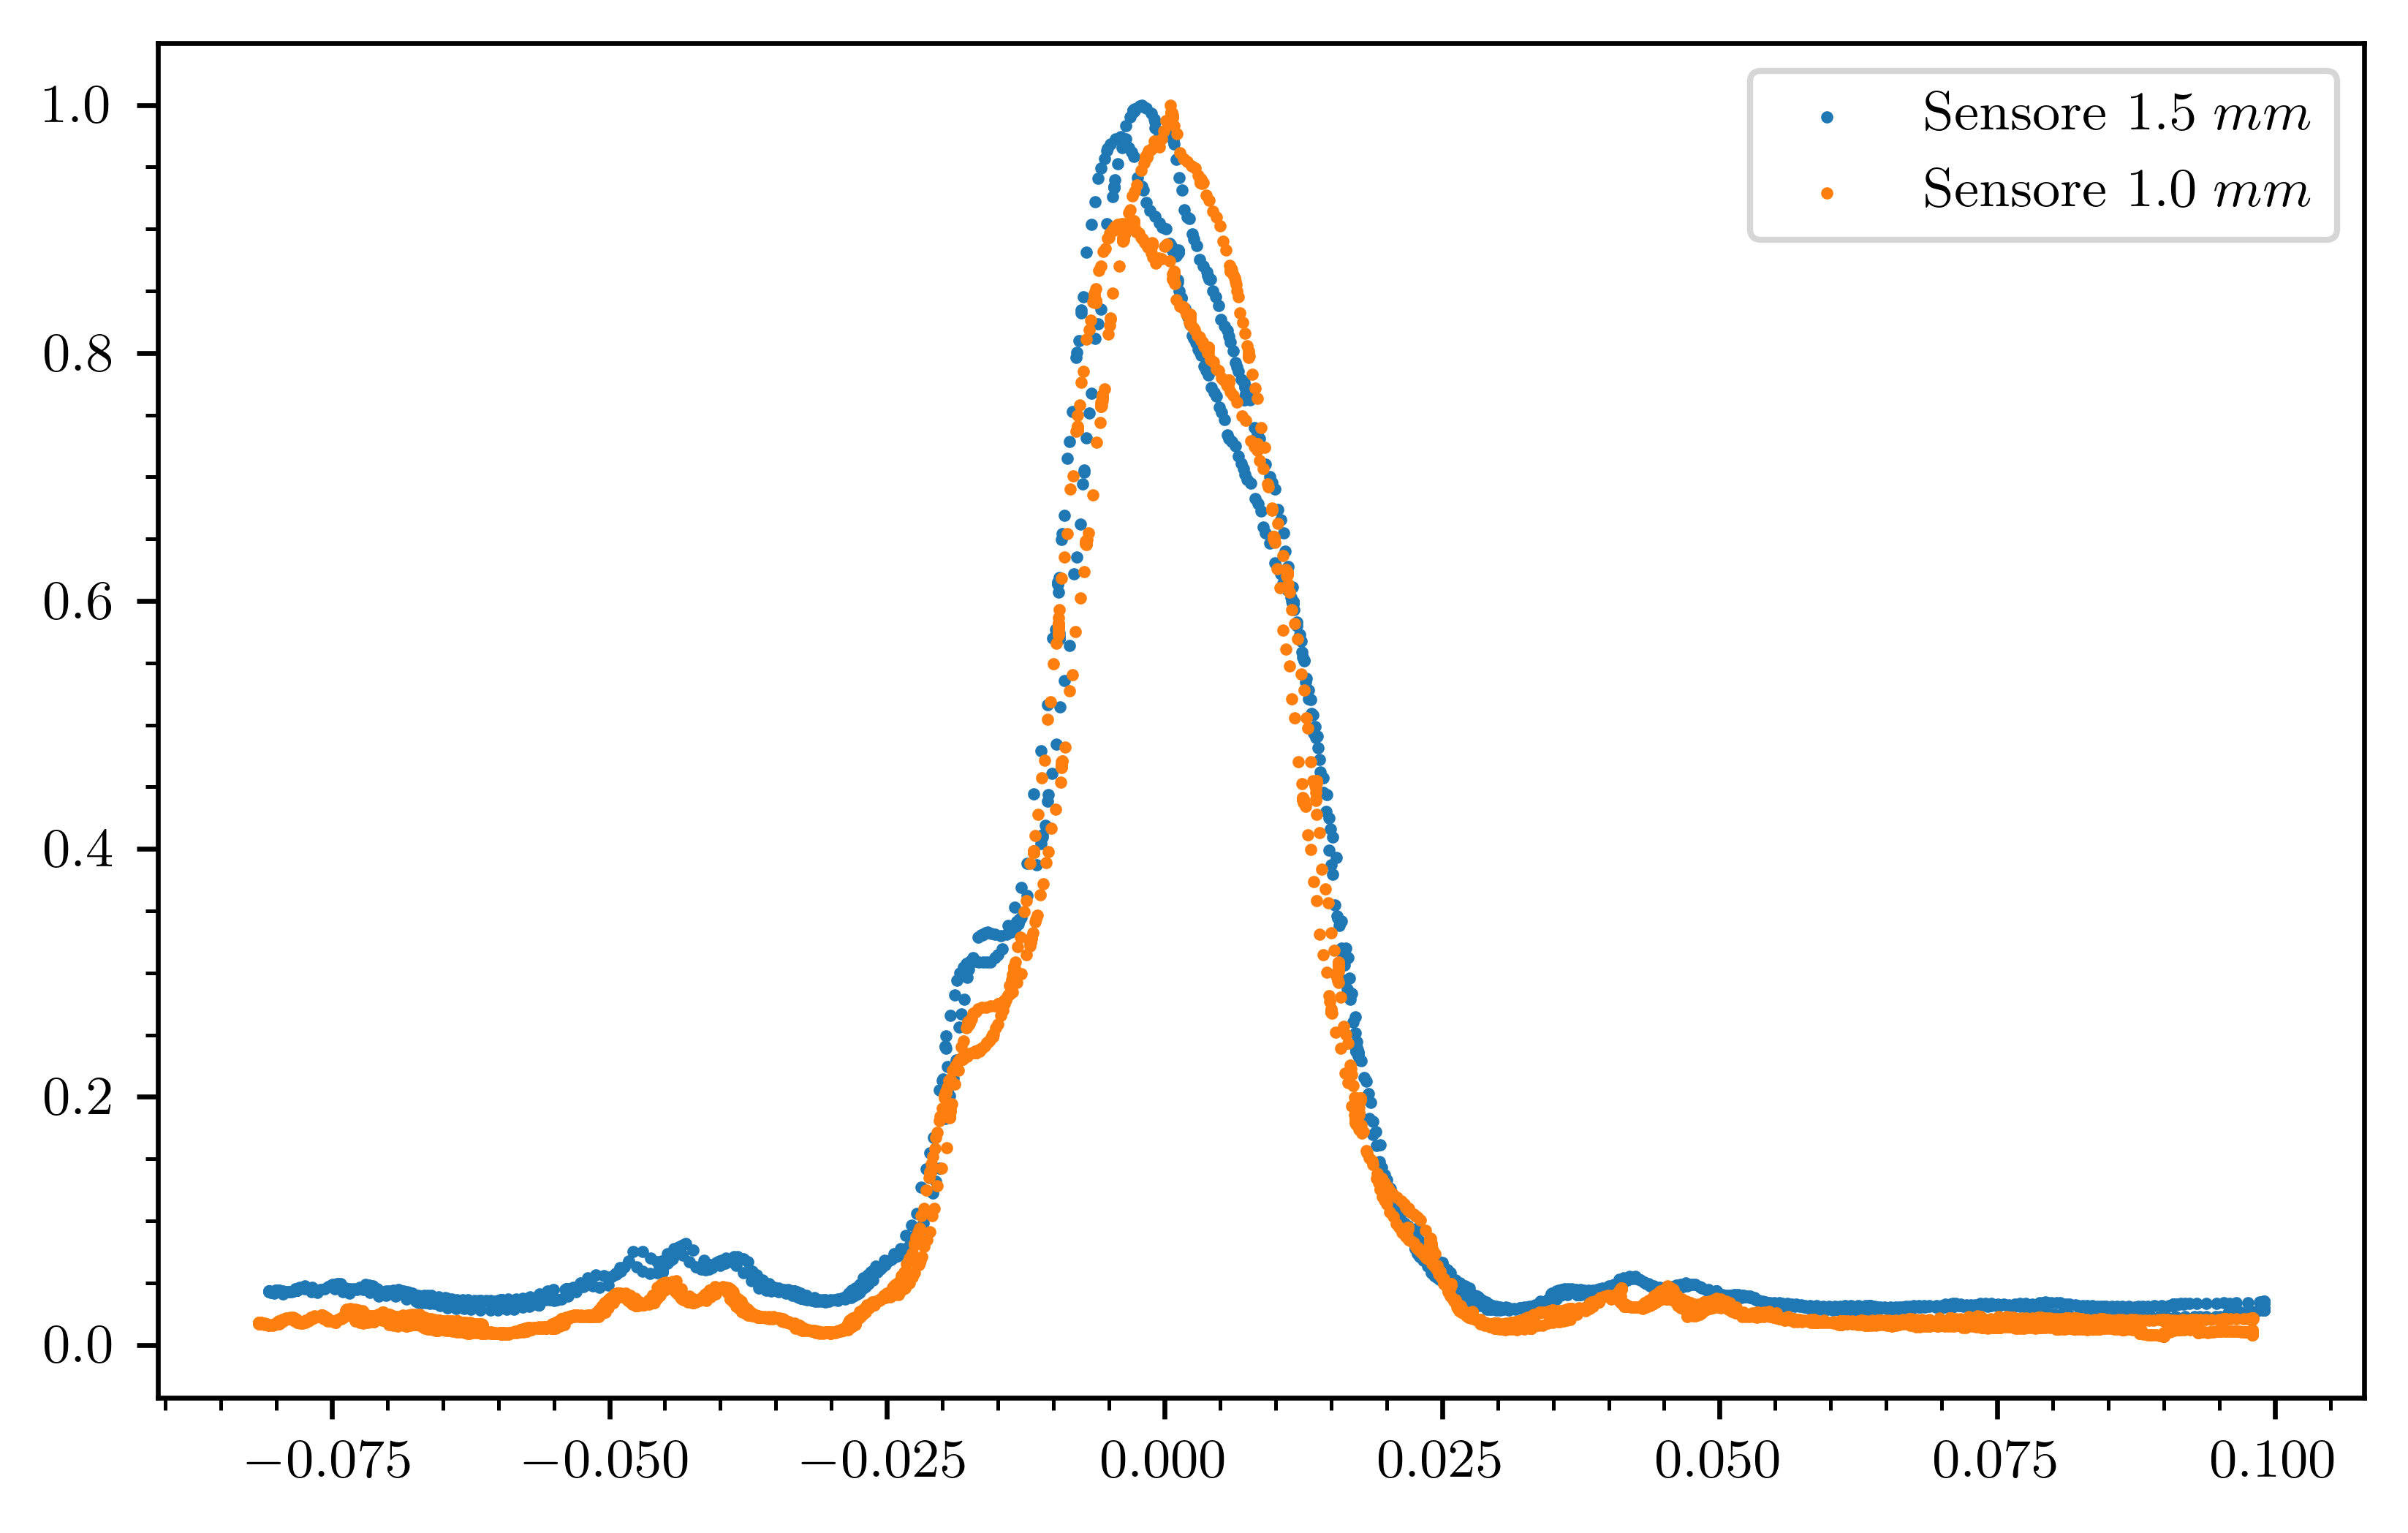
\includegraphics{sensor_0.02.png}
    \caption{Grafico dell'intensità luminosa relativa $I$ in funzione della posizione $y$ (in metri) per ciascuna delle due aperture del sensore.
        Riducendo l'apertura del sensore l'intensità misurata diminuisce permettendo di passare al fondo-scala più piccolo (\textit{candela}) per l'apertura da $\qty{1.0}{\mm}$.
        I valori delle intensità sono stati scalati in modo che l'altezza del picco centrale fosse pari a $1$, questo permette di confrontare i picchi con più semplicità. In effetti è possibile notare come la curva tracciata dalle misure con un'apertura più stretta abbia un picco centrale leggermente più schiacciato.
        Inoltre nelle code delle curve è evidente come il rumore di fondo diminuisca notevolmente, in particolar modo nel set di dati con il sensore a $\qty{1.0}{\mm}$. Questo potrebbe essere dovuto alla riduzione della luce che entra nel sensore o al cambio di fondo-scala, che porta ad una corrente di buio notevolmente inferiore.
        Come sarà possibile vedere in seguito la seconda ipotesi è quella che più si adatta ai dati raccolti.} %! quantificare di quanto si stringe il picco
    \label{fig:sensore 0.02}
\end{figure}

Si può notare che anche nei grafici \ref{fig:minimi 0.02} e \ref{fig:sensore 0.02} persiste il segnale di frequenza costante: questo potrebbe essere dato da un difetto della fenditura stessa, che causa un'interferenza la quale si sovrappone alla figura di diffrazione.


\end{document}